% Chapter 3
% 
\chapter{Project Planning} % Main chapter title

%-------------------------------------------------------------------------------
%---------

\section{Project Charter}

The project charter provides a overview of the stakeholders, benefits, and assumptions of the project to state the begin of the project.

\noindent \textbf{Stakeholder}

\begin{table}[h!]
      \centering
      \begin{tabular}{|p{11cm}|c|c|}
            \hline
            \textbf{Identification}                                                         & \textbf{Power} & \textbf{Interest} \\ \hline
            Students and developers in the areas of distributed systems and fault tolerance & Low            & Medium            \\ \hline
            Administration of the master's program, responsible for dissertation evaluation & Medium         & Medium            \\ \hline
            Advisor                                                                         & High           & High              \\ \hline
      \end{tabular}
\end{table}

The administration of the master's degree programme exerts a moderate influence due to the necessity of complying with institutional requirements. Also, there is potential interest in the results, given that it will be a project for the institution. In contrast, the advisor exerts a high level of influence and interest, as his guidance and approval are fundamental to the success of the project. Furthermore, students and developers in general have an interest in the outcome of this project, considering it to be a guide for a better choice related to the fault tolerance aspects, but they exert low influence.

\textbf{Benefits}

\begin{itemize}
      \item \textbf{Decision Support for Developers:}
            The project will provide a detailed analysis of fault tolerance aspects in Elixir, Go, and Scala with Akka, offering developers and system architects a practical guide to help them choose the most suitable language for specific fault-tolerant distributed systems scenarios.

      \item \textbf{Open Source Opportunities:}
            The findings could reveal areas for improvement in the evaluated languages, inspiring open-source developers to create libraries, frameworks, or enhancements to already existing ones.

      \item \textbf{Academic Contributions:}
            The dissertation will contribute to the existing body of knowledge in the areas of distributed systems, fault tolerance, and microservices. It will provide insights into comparative aspects in the languages of debate.

\end{itemize}

\noindent \textbf{Assumptions}

\begin{itemize}
      \item \textbf{Computational Resources:}
            It is assumed that the available computational resources, including hardware and software tools, will suffice to simulate the benchmarking scenarios for each language under realistic system conditions.

      \item \textbf{Support and Guidance:}
            The advisor will provide timely and effective feedback on each deliverable, ensuring alignment with project objectives.

      \item \textbf{Consistency Across Languages:}
            The chosen languages (Elixir, Go, Scala with Akka) have sufficient community support, libraries, and tools to implement the required benchmarking scenarios consistently.
\end{itemize}

\section{Work Breakdown Structure}

The objective of the \gls{WBS} is to detail the project scope in a visual and hierarchical manner, enabling a clear understanding of how each deliverable connects to the overall project.
% \footnote{WBS Practice Standard: \url{https://www.projectmanagement.com/deliverables/311939/work-breakdown-structure–wbs–practice-standard-package/} (accessed 30 November 2024)}. 
As shown in Figure \ref{fig:wbs}, the main point of this project is the dissertation. With the objective defined, the first phase focuses on project planning. This phase establishes the foundation by outlining the project charter, creating a \gls{WBS}, and developing a timeline through a Gantt chart.

Once the planning phase is complete, the subsequent phases align with the Design and Creation research method. This research method was chosen given the nature of the project, because while the final objective is clear, there are uncertainties about how to achieve each stage, as every step builds on the outcomes of the previous one. Consequently, the method divides the project into sequential phases: design, implementation, and conclusion. Each phase has clearly defined deliverables that align with the \gls{WBS}, ensuring that progress can be monitored and adjustments can be made as needed.

The final phase, the conclusion, consolidates all findings and results, translating them into the completed dissertation.


\begin{figure}
      \centering
      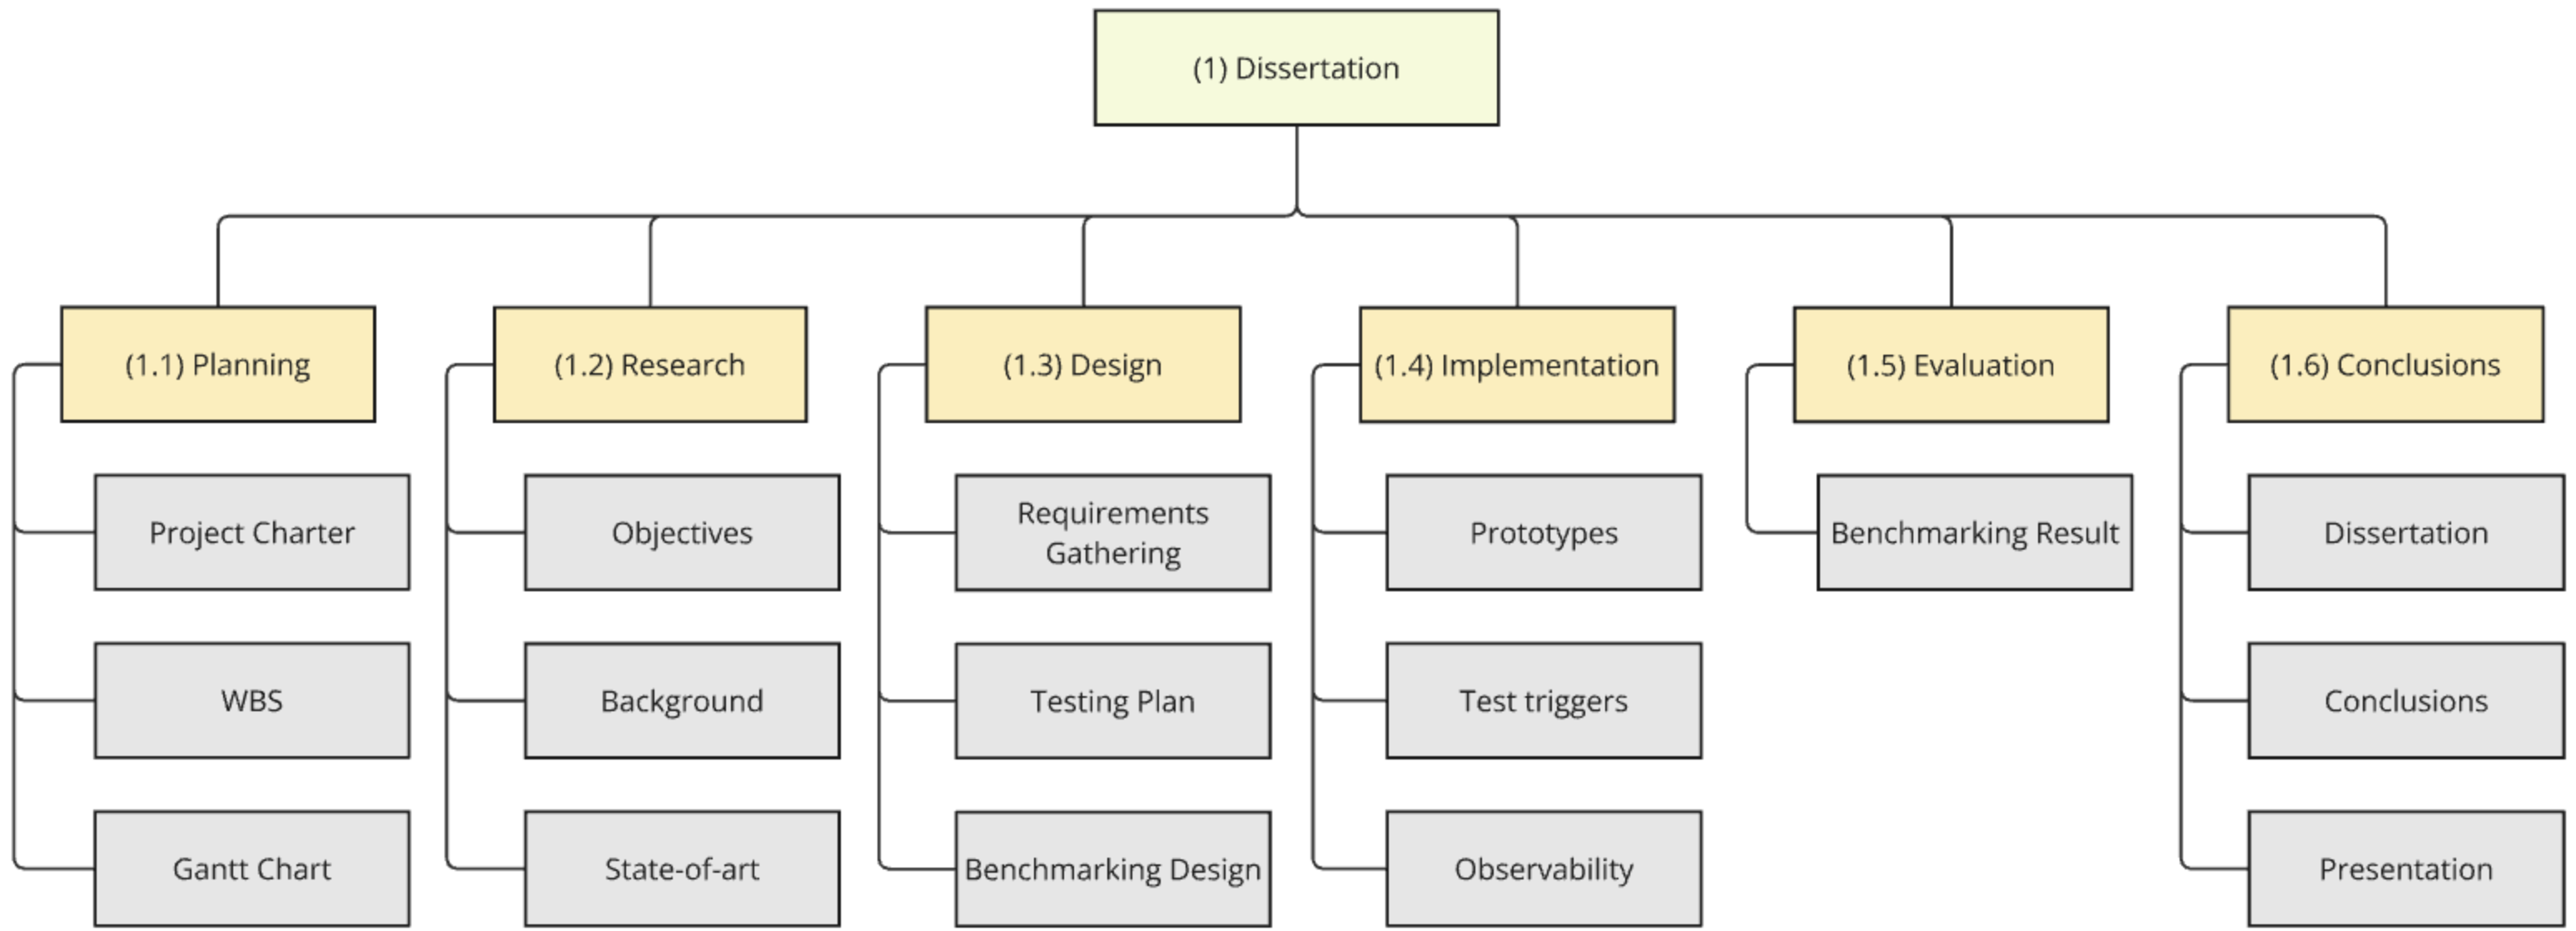
\includegraphics[width=\linewidth]{ch-planning/assets/wbs.png}
      \caption{The \gls{WBS} of the project.}
      \label{fig:wbs}
\end{figure}


\textbf{Work Breakdown Structure Dictionary.} Following is described the \gls{WBS} Dictionary that as the responsibility of detailing each phase in order to be defined what are the goals and the acceptance criteria in a concise and clear way.

\begin{longtable}{|p{3cm}|p{2.5cm}|p{8cm}|}
      \hline
      \textbf{Item Name}             & \textbf{Type of Item} & \textbf{Additional Description / Acceptance Criteria}                                                                                                                                                                                                                                                                                                     \\ \hline
      \endfirsthead
      \hline
      \textbf{Item Name}             & \textbf{Type of Item} & \textbf{Additional Description / Acceptance Criteria}                                                                                                                                                                                                                                                                                                     \\ \hline
      \endhead
      (1.1) Planning                 & Phase                 & This phase includes all initial project setup tasks.                                                                                                                                                                                                                                                                                                      \\ \hline
      (1.1.1) Project Charter        & Deliverable           & The project charter must be created following the project's scope and management guidelines. \newline \textbf{Acceptance Criteria:} The project charter must be approved by the advisor.                                                                                                                                                                  \\ \hline
      (1.1.2) \gls{WBS}              & Deliverable           & The \gls{WBS} should break down the project into manageable components. \newline \textbf{Acceptance Criteria:} The WBS should be validated by the advisor and include all project elements.                                                                                                                                                               \\ \hline
      (1.1.3) Gantt Chart            & Deliverable           & A detailed timeline outlining tasks, dependencies, competence development plan, milestones, and the dissertation deadline. \newline \textbf{Acceptance Criteria:} The Gantt chart must accurately reflect project phases and be reviewed by the advisor.                                                                                                  \\ \hline
      \hline % Separator between phases

      (1.2) Research                 & Phase                 & This phase focuses on gathering the required knowledge and literature to support the project.                                                                                                                                                                                                                                                             \\ \hline
      (1.2.1) Objectives             & Deliverable           & Clear objectives for the project, that must detail what are the excepted outcomes. \newline \textbf{Acceptance Criteria:} Objectives should align with the research goals and be validated by the advisor.                                                                                                                                                \\ \hline
      (1.2.2) Background             & Deliverable           & Research and summarize the background of fault tolerance in distributed systems and the distributed and concurrent programming languages.  \newline \textbf{Acceptance Criteria:} The background section should include sufficient theoretical content approved by the advisor, and must include a clear justification for the languages chosen.          \\ \hline
      (1.2.3) State-of-art           & Deliverable           & Review the current literature on fault tolerance in Elixir, Go, and Scala with Akka. Also, what are the latest techniques for benchmarking distributed and concurrent programming, and if there are already studies on this topic. \newline \textbf{Acceptance Criteria:} State-of-the-art review must highlight gaps and relevance to the project scope. \\ \hline
      \hline % Separator between phases

      (1.3) Design                   & Phase                 & This phase involves requirements gathering, testing plan, and benchmarking design.                                                                                                                                                                                                                                                                        \\ \hline
      (1.3.1) Requirements Gathering & Deliverable           & Collect requirements for the benchmarking and evaluation of fault tolerance aspects. \newline \textbf{Acceptance Criteria:} Requirements must be detailed, reviewed, and approved by the advisor.                                                                                                                                                         \\ \hline
      (1.3.2) Testing Plan           & Deliverable           & A plan for testing different fault tolerance strategies and mechanisms in Elixir, Go, and Scala with Akka. \newline \textbf{Acceptance Criteria:} Testing plan must include scenarios and validation methods, reviewed by the advisor.                                                                                                                    \\ \hline
      (1.3.3) Benchmarking Design    & Deliverable           & Define the design for benchmarking environments. \newline \textbf{Acceptance Criteria:} Benchmarking environments design must be validated by the advisor, and must adhere to the test plan created.                                                                                                                                                      \\ \hline
      \hline % Separator between phases

      (1.4) Implementation           & Phase                 & This phase involves the development of benchmarking prototypes.                                                                                                                                                                                                                                                                                           \\ \hline
      (1.4.1) Prototypes             & Deliverable           & Develop prototypes in Elixir, Go, and Scala with Akka for fault tolerance testing. \newline \textbf{Acceptance Criteria:} Prototypes must meet the test plan previously created and must be supported on the benchmarking design planned.                                                                                                                 \\ \hline
      (1.4.2) Test Triggers          & Deliverable           & Create fault injection mechanisms for testing fault tolerance. \newline \textbf{Acceptance Criteria:} Fault injection methods must simulate real-world scenarios and be validated by tests.                                                                                                                                                               \\ \hline
      (1.4.3) Observability          & Deliverable           & Implement observability tools for monitoring system behavior during tests. \newline \textbf{Acceptance Criteria:} Observability setup must capture the metrics defined on the test validations methods.                                                                                                                                                   \\ \hline
      \hline % Separator between phases

      (1.5) Evaluation               & Phase                 & Evaluate the results of the benchmarking tests.                                                                                                                                                                                                                                                                                                           \\ \hline
      (1.5.1) Benchmarking Result    & Deliverable           & Analyze and document the outcomes of benchmarking fault tolerance aspects. \newline \textbf{Acceptance Criteria:} Results must be clear, reproducible, and reviewed by the advisor.                                                                                                                                                                       \\ \hline
      \hline % Separator between phases

      (1.6) Conclusions              & Phase                 & Finalize and present the results of the dissertation.                                                                                                                                                                                                                                                                                                     \\ \hline
      (1.6.1) Dissertation           & Deliverable           & Compile the dissertation document with findings and analyses. \newline \textbf{Acceptance Criteria:} Dissertation must meet academic formatting and content guidelines.                                                                                                                                                                                   \\ \hline
      (1.6.2) Conclusions            & Deliverable           & Write concise conclusions summarizing key findings from the research, with the goal of creating a guide for future developers consult. \newline \textbf{Acceptance Criteria:} Conclusions must be concise and detail what are the cons and pros of using each language for each specific case, so that develops can easily decide.                        \\ \hline
      (1.6.3) Presentation           & Deliverable           & Prepare and deliver the final presentation to the evaluation committee. \newline \textbf{Acceptance Criteria:} Presentation must be clear and precise.                                                                                                                                                                                                    \\ \hline
      \caption{\gls{WBS} dictionary}
\end{longtable}

\section{Gantt Diagram}

This section relates the details of the gantt diagram. The gantt diagram it was done on the Microsoft Project, and its timeline it is possible to observe on Figure \ref{fig:gantt_timeline}. For simplicity it is only shown the main phases, the milestones, and the periodically of the control and feedback meetings. Also, the time that the development of competencies it will cover in terms of tasks. The detailed information it will be described bellow. This gives an overview and sees that the organization of thr project its mateched wiht the \gls{WBS}. However, for further detail, on the AppendixA section of the planning is displayed on the Appendix Chapter \ref{AppendixA}. \todo{texto e appendix}

\begin{figure}
      \centering
      \frame{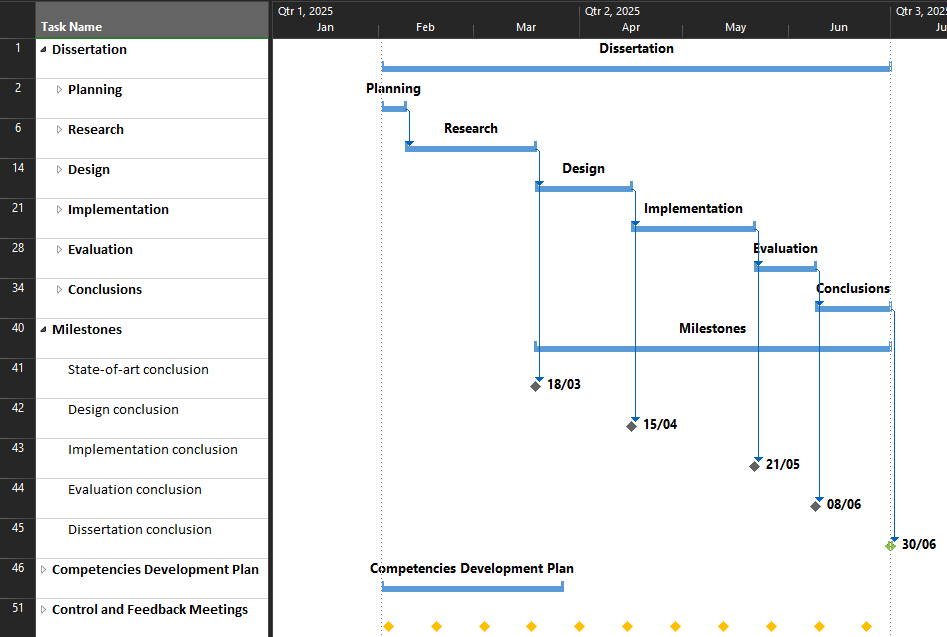
\includegraphics[width=\linewidth]{ch-planning/assets/gantt_timeline.png}}
      \caption{Gantt timeline of the project}
      \label{fig:gantt_timeline}
\end{figure}


\subsection{Project Management and Scheduling}

For the project management, the start date was set to 02/02/2025, after the first semester exams, and the end date to the predefined date associated with the project of 30/06/2025, like illustrated in Figure \ref{fig:gantt_timeline}. The scheduling strategy is to use the automatic mode where it calculates the dates based on the days of each task and the relationship between them, leveraging on the estimation on days. The schedule is based on a calendar with no restrictions on working days, meaning all days, including weekends, are considered working days to ensure continuous progress.

\todo[inline]{melhorar esta parte de baixo}

\textbf{Estimation Rationale.} Task duration estimates were determined based on the complexity and importance of each phase. The background and state-of-the-art sections were assigned the highest weights due to their critical role in forming the foundation of the research. These sections require extensive literature review and analysis, which are time-intensive. After completing the research phase, the design stage was given significant weight, as it involves defining requirements and developing a comprehensive testing plan, both of which are essential for a successful implementation.

The duration of the implementation phase was estimated considering the iterative nature of prototyping and testing triggers, ensuring sufficient time for observability and adjustments. The evaluation phase, particularly benchmarking results, was scheduled with adequate time to ensure thorough analysis and interpretation of the findings. Lastly, the conclusions phase was planned with sufficient time to synthesize the project outcomes and finalize the dissertation.

\textbf{Resource Allocation and Monitoring.} A resource table was included in the project plan to track resource allocation, focusing on the student and advisor as the primary stakeholders. The advisor’s role is focused on controlling and monitoring tasks, providing feedback and guidance throughout the project.

\textbf{Cost Management.} The cost component was excluded from the project plan, as it is not applicable to this type of academic project.

\subsection{Monitoring and Controlling Procedures}

The strategy defined to have control over the progress of each task was to mark its progress by an estimated percentage of completion. This strategy ensures that the progress of the task is clearly visible and measurable, giving both the student and the advisor a view of progress, like it is possible to observe the “\% Completed” column on the Figure \ref{fig:gantt_monitoring}.

To improve this process, specific tasks dedicated to monitoring and control have been incorporated, such as \textit{“Validation and Refinement with the Advisor”}, like illustrated on Figure \ref{fig:gantt_monitoring}. These tasks have two main objectives, firstly, to make the student responsible for presenting the partial document ready to be assessed. Secondly, to ensure that the advisor is warned in advance of the need for closer and more active feedback on these pre-defined days. Feedback can be given asynchronously via messages or synchronously during scheduled meetings. After the feedback time is up, the goal is to be able to present a refined partial document, referred to as the \textit{“Document version X”} task, also possible to observe on Figure \ref{fig:gantt_monitoring}.

\begin{figure}
      \centering
      \frame{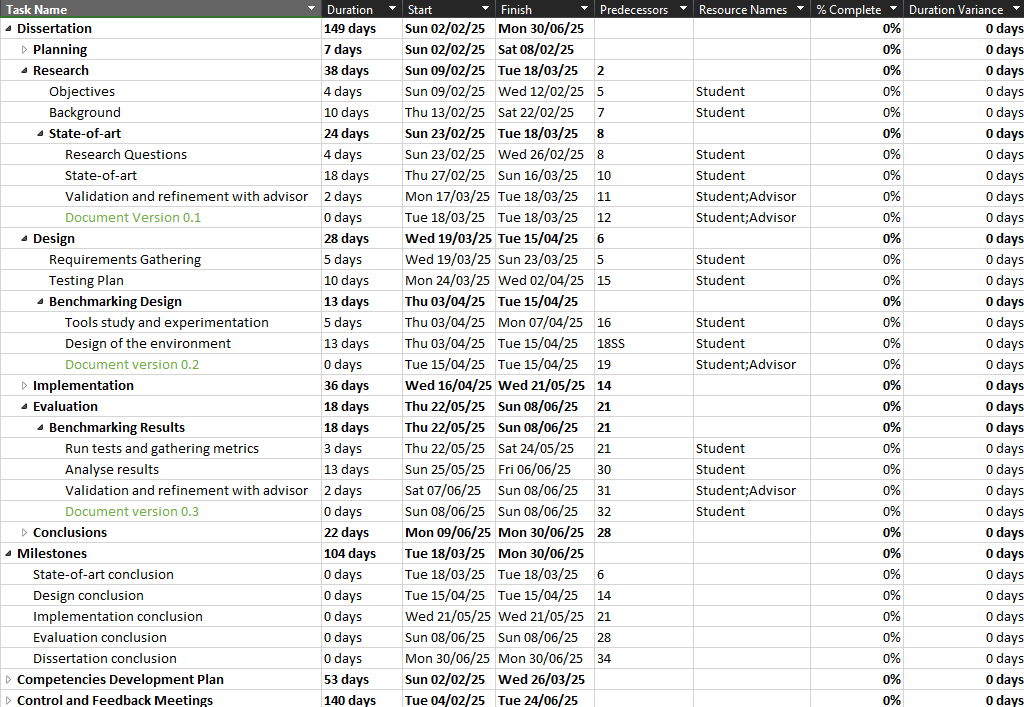
\includegraphics[width=\linewidth]{ch-planning/assets/gantt_monitoring.png}}
      \caption{Monitoring and control procedures displayed on the Gantt chart.}
      \label{fig:gantt_monitoring}
\end{figure}

Additionally, milestones have been defined to mark the completion of each significant project phase. These milestones serve as checkpoints to ensure progress is on track and can be observed in Figure \ref{fig:gantt_monitoring} under the main task \textit{“Milestones”}.

To manage potential delays, a baseline has been established. This baseline records the initial schedule, allowing deviations to be tracked throughout the project. This mechanism provides an overview of delays and their impact on the schedule. The \textit{“Column Variance”} column in Figure \ref{fig:gantt_monitoring} illustrates this feature, allowing a visualization of changes between planned and actual progress.

\subsection{Meeting Sessions}

To ensure consistent communication and effective progress monitoring with the advisor, a series of biweekly meetings has been scheduled on Wednesdays, with each session expected to last between 30 minutes and 1 hour. While the schedule includes a predefined list of sessions, it remains flexible, allowing adjustments to the frequency of meetings as the project evolves. For instance, the number of meetings may increase during the final stages of the project, at which point the Gantt chart will be updated accordingly.

\begin{figure}
      \centering
      \frame{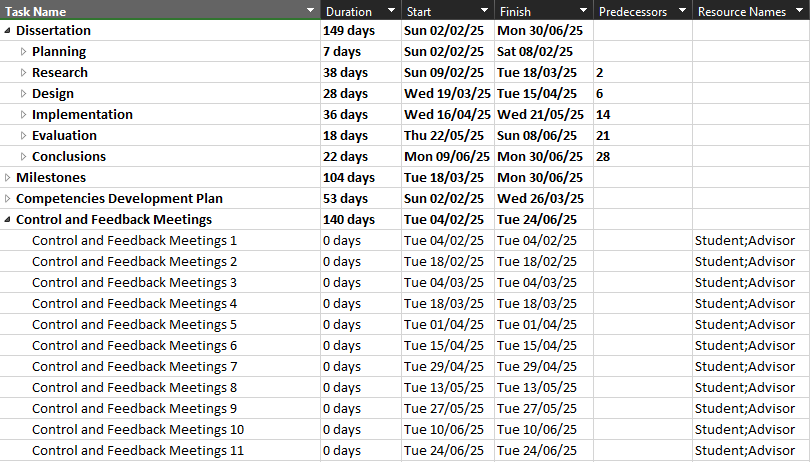
\includegraphics[width=\linewidth]{ch-planning/assets/gantt_meetings.png}}
      \caption{Meeting sessions represented on the Gantt chart.}
      \label{fig:gantt_meetings}
\end{figure}

The meeting schedule is illustrated in Figure \ref{fig:gantt_meetings}, which includes 11 recurring tasks organized under the main task \textit{“Meeting Sessions”}. These meetings are planned to take place online.

\subsection{Competencies Development Plan}

To address the competencies identified during the diagnosis of critical skills required for the completion of the dissertation, a dedicated section titled \textit{"Competencies Development Plan”} has been incorporated into the project plan, as illustrated in Figure \ref{fig:gantt_competency}. This section outlines targeted tasks designed to address these areas for improvement.

\begin{figure}
      \centering
      \frame{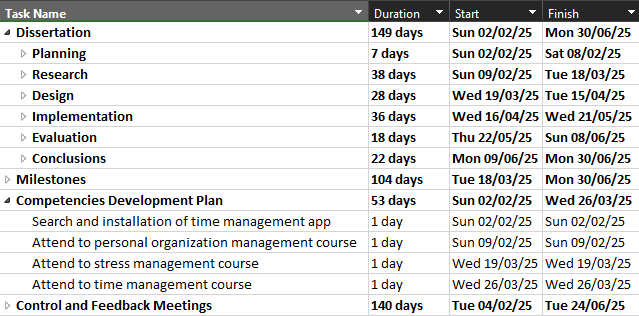
\includegraphics[width=\linewidth,scale=0.5]{ch-planning/assets/gantt_skills.png}}
      \caption{Competencies development plan represented on the Gantt chart.}
      \label{fig:gantt_competency}
\end{figure}

For stress management and resilience, the plan includes attending a Stress Management course.
\footnote{Managing Stress Course: \url{https://www.linkedin.com/learning/managing-stress-2019/} (accessed 4 December 2024)}. To enhance self-discipline and time management, the initial task involves identifying and installing at least one productivity application, such as tools that restrict smartphone usage during certain periods, for example. Additionally, time management competence is further explored by taking the Time Management Fundamentals course
\footnote{Time Management Fundamentals Course: \url{https://www.linkedin.com/learning/time-management-fundamentals-14548057/the-power-of-managing-your-time/} (accessed 4 December 2024)}.

Communication, another key area of focus, will be developed by attending to the "Communicating with Confidence" course
\footnote{Communicating with Confidence Course: \url{https://www.linkedin.com/learning/como-se-comunicar-com-confianca/} (accessed 4 December 2024)}.

\section{Risk Management}

Effective risk management seeks to transform potential uncertainties into more predictable and controlled outcomes. To achieve this, the most significant risks identified are described next

\subsection{Risk 1: Bugs in Third-Party Libraries}

\textbf{Description:} There is a potential risk of encountering bugs in third-party libraries, which could compromise the viability of implementation and testing of the prototypes. Since the project relies on external libraries to implement fault-tolerant strategies, the stability and reliability of these libraries are important.

\textbf{Cause:} The cause of this risk is the need of trust on external software components.

\textbf{Effect on the Project:} Errors in the libraries can compromise the viability of the prototype's development and also the integrity of the results.

\textbf{Risk Owner:} Student.

\textbf{Probability.} 2. \textbf{Impact:} 4. \textbf{PI Score.} 8.

\textbf{Risk Response Strategy:} To mitigate this risk, alternative libraries will be identified for each strategy and language in advance. At least two or three libraries will be shortlisted and prioritized. If the primary library encounters significant bugs or issues, the next library on the list will be utilized.

\textbf{Expected Result Without Action:} If no action is taken, delays in prototype development will occur.

\textbf{Risk Response Type:} Mitigation.

\textbf{Response Description:} A proactive approach will be taken to evaluate multiple libraries during the research phase.


\subsection{Risk 2: Integration Challenges Between Components}

\textbf{Description:} Integration issues could arise when combining multiple components, such as third-party libraries, testing frameworks, and custom implementations.

\textbf{Cause:} Differences in interfaces, versions, or dependencies among components used in the project.

\textbf{Effect on the Project:} These challenges could delay testing and result in compatibility issues that reduce productivity.

\textbf{Risk Owner:} Student.

\textbf{Probability.} 2. \textbf{Impact:} 4. \textbf{PI Score.} 8.

\textbf{Risk Response Strategy:} To mitigate this risk, dependencies and versions will be carefully managed using dependency management tools (e.g., \textit{mix} for Elixir, \textit{go.mod} for Go,  \textit{sbt} for Scala). Component integration will also be tested incrementally to identify issues early.

\textbf{Expected Result Without Action:} Significant delays during the integration phase.

\textbf{Risk Response Type:} Mitigation.

\textbf{Response Description:} Incremental integration and version control practices will ensure smoother component interaction.